During the training with PCC loss the model has successfully converged already after 35 epochs, however a clear overfit was encountered (see Figure \ref{fig:er-overfit} [left]) with the best PCC loss before the overfit being $0.0713$. Overfitting happens due to the lack of data, as for the case of ER there were much fewer samples than for nuclei for example (see Table \ref{table:data}). Even though one could use early-stopping approach and simply choose an earlier epoch before overfit, the better approach would be to use regularization methods described in section \ref{section:regularization}. Additional regularization in terms of data augmentations was introduced. The new learning curve is shown in Figure \ref{fig:er-overfit} (middle). Overfit now happens much later (after $120$ epochs) and PCC loss improves to $0.0701$. Introducing a stronger regularization with the use of weight decay in adadelta optimizer and dropout layers with a dropout rate of $0.1$ (see Figure \ref{fig:er-overfit} [right]) reduces the overfit completely, however at the same time increases the loss to $0.099$.
\begin{figure}[H]
	\begin{center}
		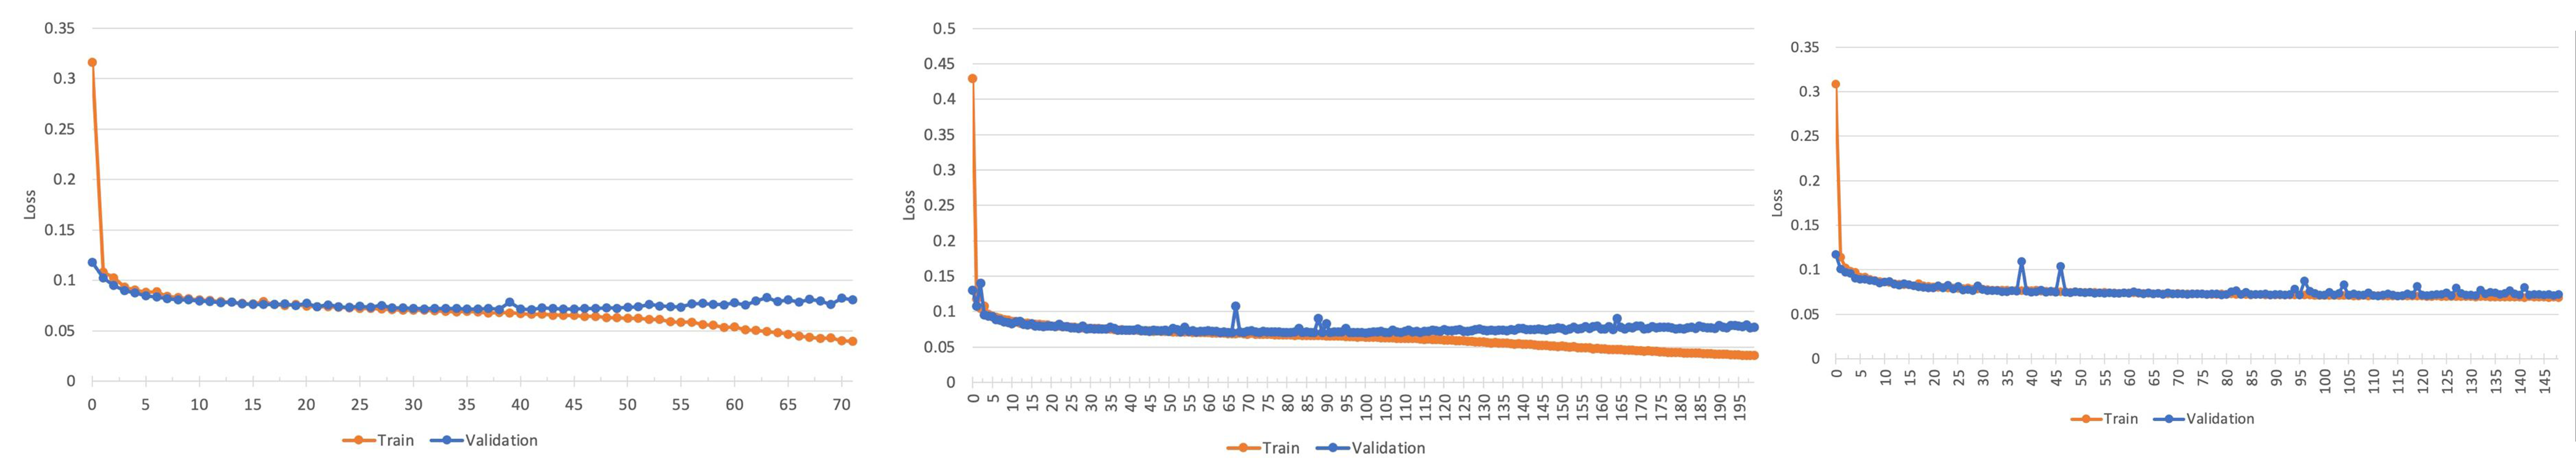
\includegraphics[width=\linewidth]{bilder/ER/segmentation/reg-not-reg.png}
		\caption{Default model (left), slightly regularized model (middle), strongly regularized model (right)}\label{fig:er-overfit}
	\end{center}
\end{figure}

Although the validation loss seems to be higher in comparison to $0.0701$, in this case the growths were not explained by the difference between the validation sets, where the loss was measured on. PCC losses on the same validation set for both were $0.0701$ and $0.0742$. It might have been the case that the regularization was too strong. In this case it would be better to use early-stopping approach with the epoch that has the lowest loss.